\section{Editor}

Di seguito vengono elencati i \glossaryItem{casi d'uso} per l'editor.

\subsection{Casi d'Uso}


\subsubsection{Operazioni ad alto livello - Uso dell'editor}
   %1) The professor says: delete the actors which don't take part to the diagram
    \begin{figure}[H]
      \begin{center}
        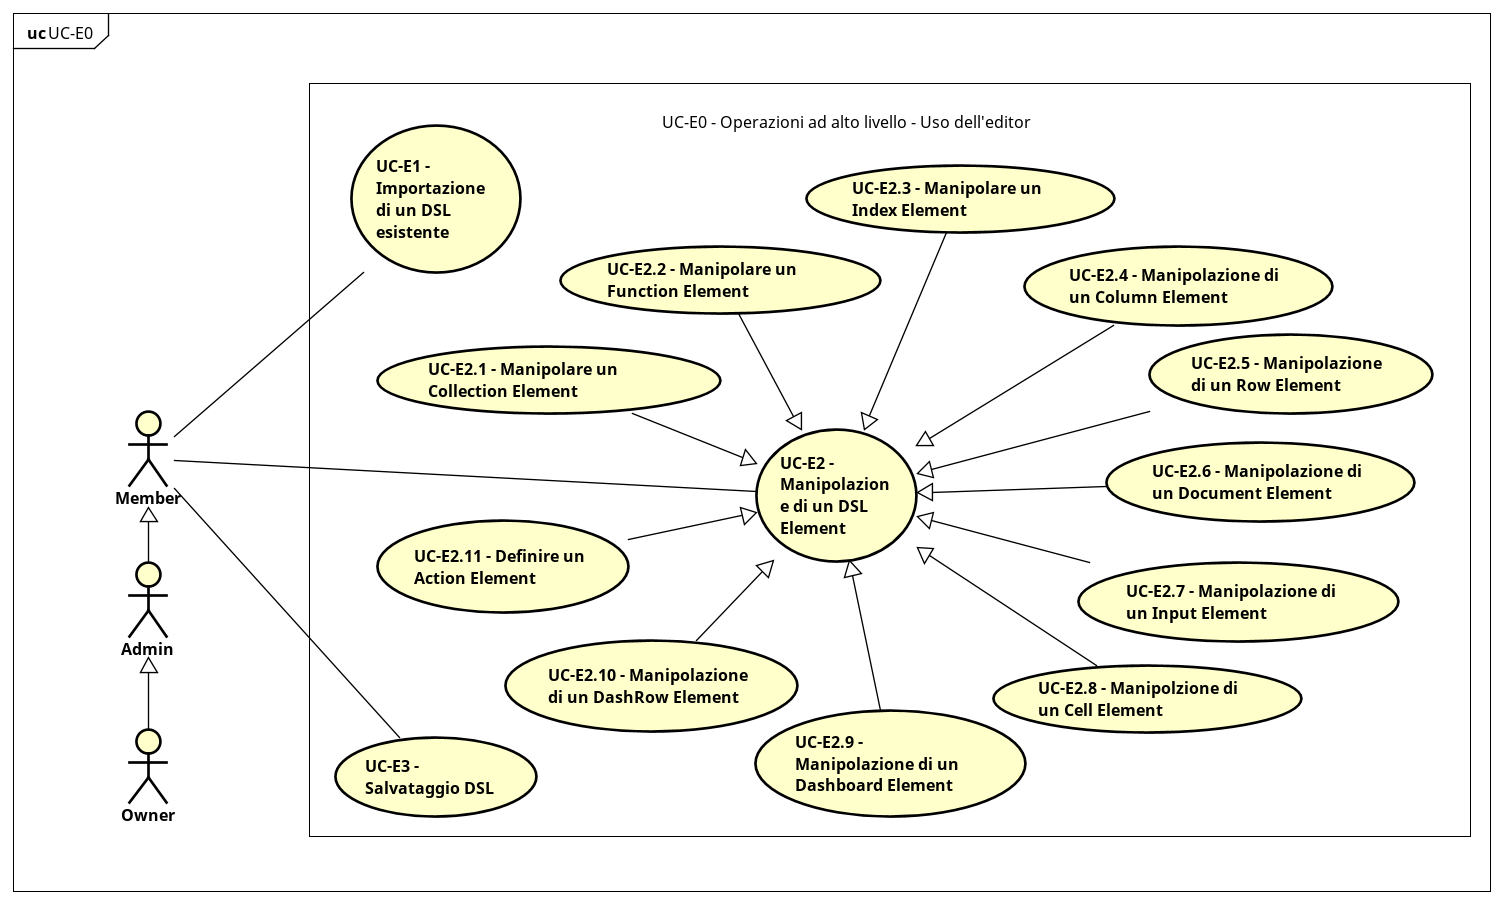
\includegraphics[width=12cm]{res/img/UCEditor/UC-E0.png}
      \caption{UC-E0 - Operazioni ad alto livello - Uso dell'editor}
      \end{center} 
    \end{figure}    
    
    %Tabella 
    \begin{center}
      \bgroup
      \def\arraystretch{1.8}     
      \begin{longtable}{  p{3.5cm} | p{8cm} } 
        
        \hline
        \multicolumn{2}{ | c | }{ \cellcolor[gray]{0.9} \textbf{UC-E0 - Operazioni ad alto livello - Uso dell'editor}} \\ 
        \hline
        
        \textbf{Attori Primari} &  \glossaryItem{Member}, \glossaryItem{Admin}, \glossaryItem{Owner} \\ 
        \textbf{Scopo e Descrizione} & L'utente visualizza l'interfaccia dell'editor tramite cui pu\`o svolgere operazioni di importazione di specifiche \glossaryItem{DSL} esistenti, manipolazione dei \glossaryItem{DSL Element} e salvataggio del \glossaryItem{DSL} corrente
        \\
        \textbf{Precondizioni}  & L'applicazione apre l'interfaccia grafica dell'editor. \\ 
        
        \textbf{Postcondizioni} & L'utente ha utilizzato l'editor ed ha eseguito le azioni volute. \\ 
        \textbf{Scenario principale} & 1. L'utilizzatore pu\`o importare una specifica \glossaryItem{DSL} esistente. (UC-E1)
        
2. L'utente pu\`o manipolare un \glossaryItem{DSL Element}. (UC-E2)

3. L'utente pu\`o salvare la specifica \glossaryItem{DSL}. (UC-E3)
      \end{longtable}
      \egroup
    \end{center}

    \subsubsection{Importazione di una specifica DSL esistente}    
    
    %Tabella 
    \begin{center}
      \bgroup
      \def\arraystretch{1.8}     
      \begin{longtable}{  p{3.5cm} | p{8cm} } 
        
        \hline
        \multicolumn{2}{ | c | }{ \cellcolor[gray]{0.9} \textbf{UC-E1 - Importazione di una specifica \glossaryItem{DSL} esistente}} \\ 
        \hline
        
        \textbf{Attori Primari} &  \glossaryItem{Member}, \glossaryItem{Admin}, \glossaryItem{Owner} \\ 
        \textbf{Scopo e Descrizione} & L'utente pu\`o importare una specifica \glossaryItem{DSL} esistente tra quelli personali o quelli della \glossaryItem{Company}. \\ 
        
        \textbf{Precondizioni}  & L'applicazione fornisce la lista delle specifiche \glossaryItem{DSL} tra cui scegliere quella da importare. \\ 
        
        \textbf{Postcondizioni} & L'applicazione ha caricato con successo la specifica \glossaryItem{DSL} richiesta dall'utente. \\
        \textbf{Scenario principale} & 1. L'utente importa una specifica \glossaryItem{DSL} esistente tra quelli personali o quelli della \glossaryItem{Company}. \\
      \end{longtable}
      \egroup
    \end{center} 


\subsubsection{Manipolazione di un DSL Element}

    \begin{figure}[H]
      \begin{center}
        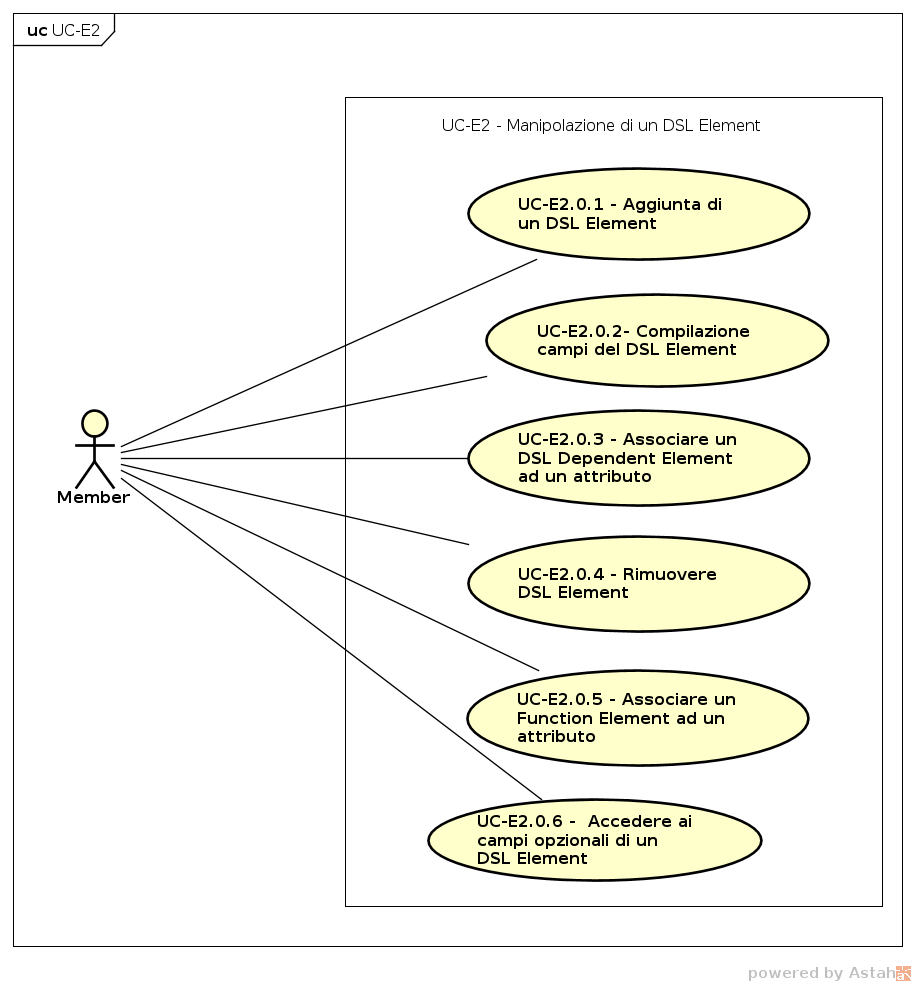
\includegraphics[width=12cm]{res/img/UCEditor/UC-E2.png}
      \caption{UC-E2 - \glossaryItem{DSL Element}}
      \end{center} 
    \end{figure}    
    
    %Tabella 
    \begin{center}
     % UC-E2: i suoi sotto-casi d’uso sono generici: come si interseca questo fatto
             %con i suoi \glossaryItem{casi} derivati? Ognuno di questi dovrebbe avere una sua
            % implementazione specifica dei suddetti. Rivedere.
      \bgroup
      \def\arraystretch{1.8}     
      \begin{longtable}{  p{3.5cm} | p{8cm} } 
        
        \hline
        \multicolumn{2}{ | c | }{ \cellcolor[gray]{0.9} \textbf{UC-E2 - Manipolazione di un \glossaryItem{DSL Element}}} \\ 
        \hline
        
        \textbf{Attori Primari} &  \glossaryItem{Member}, \glossaryItem{Admin}, \glossaryItem{Owner} \\ 
        \textbf{Scopo e Descrizione} & L'utente pu\`o creare, manipolare o rimuovere un \glossaryItem{DSL Element} all'interno dell'editor. \\ 
        
        \textbf{Precondizioni}  & L'utente visualizza l'editor. \\ 
        
        \textbf{Postcondizioni} & L'utente ha eseguito le sue operazioni sul \glossaryItem{DSL Element} con successo. \\ 
        \textbf{Scenario Principale} & 1. L'utente pu\`o aggiungere un \glossaryItem{DSL Element}. (UC-E2.0.1)
        
2. L'attore pu\`o compilare i campi informativi del \glossaryItem{DSL Element}. (UC-E2.0.2)

3. L'utente pu\`o collegare un \glossaryItem{DSL element} ad un attributo. (UC-E2.0.3)

4. L'utente ha la possibilit\`a di rimuovere un \glossaryItem{DSL Element}. (UC-E2.0.4)

5. L'utente ha la possibilit\`a di associare un \glossaryItem{Function Element} al \glossaryItem{DSL Element}. (UC-E2.0.5)

6. L'utente ha la possibilit\`a di accedere ai campi opzionali di un \glossaryItem{DSL Element}. (UC-E2.0.6)
      \end{longtable}
      \egroup
    \end{center} 


\subsubsection{Aggiunta di un DSL Element}   
    
    %Tabella 
    \begin{center}
      \bgroup
      \def\arraystretch{1.8}     
      \begin{longtable}{  p{3.5cm} | p{8cm} } 
        
        \hline
        \multicolumn{2}{ | c | }{ \cellcolor[gray]{0.9} \textbf{UC-E2.0.1 - Aggiunta di un \glossaryItem{DSL Element}}} \\ 
        \hline
        
        \textbf{Attori Primari} &  \glossaryItem{Member}, \glossaryItem{Admin}, \glossaryItem{Owner} \\ 
        \textbf{Scopo e Descrizione} & L'utente ha la possibilità di aggiungere un \glossaryItem{DSL Element} e di deciderne il tipo. \\ 
        
        \textbf{Precondizioni}  & L'utente visualizza l'editor. \\ 
        
        \textbf{Postcondizioni} & L'utente ha aggiunto con successo un \glossaryItem{DSL Element}.\\
        \textbf{Scenario principale} & 1. L'utente aggiunge un \glossaryItem{DSL Element}. \\ 
      \end{longtable}
      \egroup
    \end{center} 
    
\subsubsection{Compilazione campi del DSL Element}

    %Tabella 
    \begin{center}
      \bgroup
      \def\arraystretch{1.8}     
      \begin{longtable}{  p{3.5cm} | p{8cm} } 
        
        \hline
        \multicolumn{2}{ | c | }{ \cellcolor[gray]{0.9} \textbf{UC-E2.0.2 - Compilazione campi del \glossaryItem{DSL Element}}} \\ 
        \hline
        
        \textbf{Attori Primari} &  \glossaryItem{Member}, \glossaryItem{Admin}, \glossaryItem{Owner} \\ 
        \textbf{Scopo e Descrizione} & L'utente ha la possibilit\`a di compilare i campi informativi del \glossaryItem{DSL Element}. \\ 
        
        \textbf{Precondizioni}  & L'utente visualizza un \glossaryItem{DSL Element}. \\ 
        
        \textbf{Postcondizioni} & Le informazioni desiderate dall'utente sono state aggiunte nel \glossaryItem{DSL Element}. \\
        \textbf{Scenario principale} & 1. L'utente compila i campi informativi del \glossaryItem{DSL Element}. \\ 
      \end{longtable}
      \egroup
    \end{center}
    
\subsubsection{Associare un DSL Element ad un attributo}

    %Tabella 
    \begin{center}
      \bgroup
      \def\arraystretch{1.8}     
      \begin{longtable}{  p{3.5cm} | p{8cm} } 
        
        \hline
        \multicolumn{2}{ | c | }{ \cellcolor[gray]{0.9} \textbf{UC-E2.0.3 - Associare \glossaryItem{DSL Element} ad un attributo}} \\ 
        \hline
        
        \textbf{Attori Primari} &  \glossaryItem{Member}, \glossaryItem{Admin}, \glossaryItem{Owner} \\ 
        \textbf{Scopo e Descrizione} & L'utente ha la possibilit\`a di associare un \glossaryItem{DSL element} ad un attributo. \\ 
        
        \textbf{Precondizioni}  & L'utente seleziona un attributo e un \glossaryItem{DSL Element} da associare. \\ 
        
        \textbf{Postcondizioni} & L'utente ha collegato con successo il \glossaryItem{DSL Element} all'attributo. \\
        \textbf{Scenario principale} & 1. L'utente associa un \glossaryItem{DSL element} ad un attributo. \\
      \end{longtable}
      \egroup
    \end{center}
\subsubsection{Rimuovere un DSL Element}

    %Tabella 
    \begin{center}
      \bgroup
      \def\arraystretch{1.8}     
      \begin{longtable}{  p{3.5cm} | p{8cm} } 
        
        \hline
        \multicolumn{2}{ | c | }{ \cellcolor[gray]{0.9} \textbf{UC-E2.0.4 - Rimuovere un \glossaryItem{DSL Element}}} \\ 
        \hline
        
        \textbf{Attori Primari} &  \glossaryItem{Member}, \glossaryItem{Admin}, \glossaryItem{Owner} \\ 
        \textbf{Scopo e Descrizione} & \`E possibile rimuovere un \glossaryItem{DSL Element}. \\ 
        
        \textbf{Precondizioni}  & L'utente sta visualizzando l'editor e il \glossaryItem{DSL Element} che vuole eliminare \`e presente nell'interfaccia dell'editor. \\ 
        
        \textbf{Postcondizioni} & L'utente ha eliminato con successo il \glossaryItem{DSL Element} selezionato.\\
        \textbf{Scenario principale} & 1. L'utente rimuove un \glossaryItem{DSL Element} dall'editor. \\ 
      \end{longtable}
      \egroup
    \end{center}
\subsubsection{Associare un Function Element ad un attributo}

    %Tabella 
    \begin{center}
      \bgroup
      \def\arraystretch{1.8}     
      \begin{longtable}{  p{3.5cm} | p{8cm} } 
        
        \hline
        \multicolumn{2}{ | c | }{ \cellcolor[gray]{0.9} \textbf{UC-E2.0.5 - Associare un \glossaryItem{Function Element} ad un attributo}} \\ 
        \hline
        
        \textbf{Attori Primari} &  \glossaryItem{Member}, \glossaryItem{Admin}, \glossaryItem{Owner} \\ 
        \textbf{Scopo e Descrizione} & L'utente ha la possibilit\`a di associare un \glossaryItem{Function Element} ad un attributo selezionabile di un \glossaryItem{DSL Element}. \\ 
        
        \textbf{Precondizioni}  & L'utente visualizza il \glossaryItem{Function Element} e il \glossaryItem{DSL Element} a cui associarlo. \\ 
        
        \textbf{Postcondizioni} & L'utente ha associato con successo la \glossaryItem{Function Element} ad un attributo del \glossaryItem{DSL Element}.\\
        \textbf{Scenario principale} & 1. L'utente associa un \glossaryItem{Function Element} ad un attributo selezionabile di un \glossaryItem{DSL Element}. \\ 
      \end{longtable}
      \egroup
    \end{center}
    
    
\subsubsection{Accedere ai campi opzionali di un DSL Element}

    %Tabella 
    \begin{center}
      \bgroup
      \def\arraystretch{1.8}     
      \begin{longtable}{  p{3.5cm} | p{8cm} } 
        
        \hline
        \multicolumn{2}{ | c | }{ \cellcolor[gray]{0.9} \textbf{UC-E2.0.6 - Accedere ai campi opzionali di un \glossaryItem{DSL Element}}} \\ 
        \hline
        
        \textbf{Attori Primari} &  \glossaryItem{Member}, \glossaryItem{Admin}, \glossaryItem{Owner} \\ 
        \textbf{Scopo e Descrizione} & L'utente ha accesso ai campi opzionali di un \glossaryItem{DSL Element} e vuole renderli modificabili. \\ 
        
        \textbf{Precondizioni}  & L'utente sta visualizzando uno specifico \glossaryItem{DSL Element} con campi opzionali. \\ 
        
        \textbf{Postcondizioni} & L'utente ha reso modificabili i campi opzionali del \glossaryItem{DSL Element}. Tali campi possono essere modificati come descritto su caso d'uso UC-E2.0.2.\\
        \textbf{Scenario principale} & 1. L'utente accede ai campi opzionali di un \glossaryItem{DSL Element} e vuole renderli modificabili. \\ 
      \end{longtable}
      \egroup
    \end{center}
    
    
    
\subsubsection{Manipolazione di un Collection Element}
 

    \begin{figure}[H]
      \begin{center}
        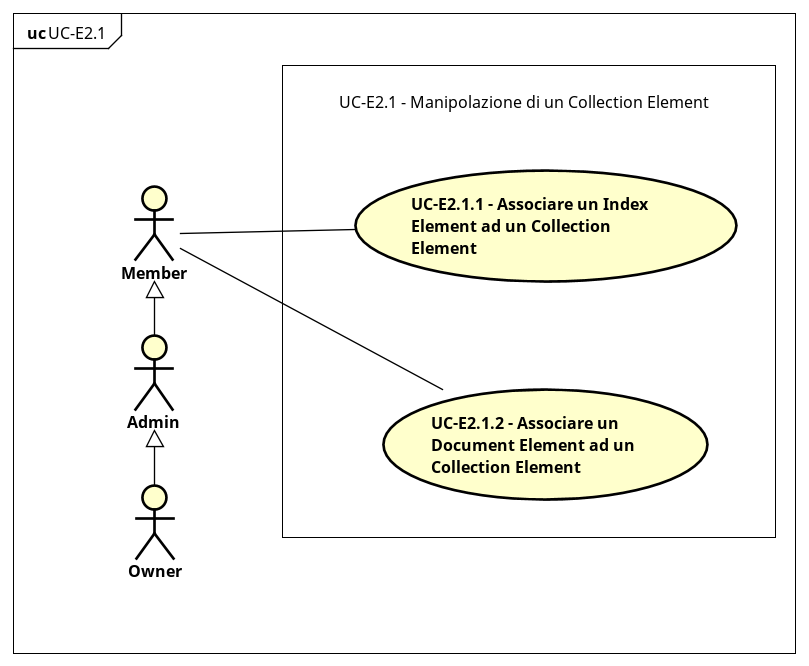
\includegraphics[width=12cm]{res/img/UCEditor/UC-E2.1.png}
      \caption{UC-E2.1 - \glossaryItem{Collection Element}}
      \end{center} 
    \end{figure}

    %Tabella 
    \begin{center}
      \bgroup
      \def\arraystretch{1.8}     
      \begin{longtable}{  p{3.5cm} | p{8cm} } 
        
        \hline
        \multicolumn{2}{ | c | }{ \cellcolor[gray]{0.9} \textbf{UC-E2.1 - Manipolazione di un \glossaryItem{Collection Element}}} \\ 
        \hline
        
        \textbf{Attori Primari} &  \glossaryItem{Member}, \glossaryItem{Admin}, \glossaryItem{Owner} \\ 
        \textbf{Scopo e Descrizione} & L'utente pu\`o creare, manipolare o rimuovere un \glossaryItem{Collection Element} all'interno dell'editor. \\ 
        
        \textbf{Precondizioni}  & L'utente sta visualizzando l'editor. \\ 
        
        \textbf{Postcondizioni} & L'utente ha manipolato il \glossaryItem{Collection Element}. \\ 
        \textbf{Scenario principale} & 1. L'utente pu\`o associare un \glossaryItem{Index Element} ad un \glossaryItem{Collection Element}. (UC-E2.1.1)
        
2. L'utente pu\`o associare un \glossaryItem{Document Element} ad un \glossaryItem{Collection Element}. (UC-E2.1.2) \\
\end{longtable}
      \egroup
    \end{center}
    
    
\subsubsection{Associare un Index Element ad un Collection Element}

    %Tabella 
    \begin{center}
      \bgroup
      \def\arraystretch{1.8}     
      \begin{longtable}{  p{3.5cm} | p{8cm} } 
        
        \hline
        \multicolumn{2}{ | c | }{ \cellcolor[gray]{0.9} \textbf{UC-E2.1.1 - Associare un \glossaryItem{Index Element} ad un \glossaryItem{Collection Element}}} \\ 
        \hline
        
        \textbf{Attori Primari} &  \glossaryItem{Member}, \glossaryItem{Admin}, \glossaryItem{Owner} \\ 
        \textbf{Scopo e Descrizione} & L'utente ha la possibilit\`a di associare un \glossaryItem{Index Element} all'attributo \glossaryItem{Index} del \glossaryItem{Collection Element}. \\ 
        
        \textbf{Precondizioni}  & Il \glossaryItem{Collection Element} a cui associare l'\glossaryItem{Index Element} \`e visualizzato nell'editor. \\ 
        
        \textbf{Postcondizioni} & L'\glossaryItem{Index Element} \`e stato associato ad un \glossaryItem{Collection Element}.\\
        \textbf{Scenario principale} & 1. L'utente associa un \glossaryItem{Index Element} all'attributo \glossaryItem{Index} del \glossaryItem{Collection Element}. \\ 
      \end{longtable}
      \egroup
    \end{center}
    
    
    
\subsubsection{Associare un Document Element ad un Collection Element}

    %Tabella 
    \begin{center}
      \bgroup
      \def\arraystretch{1.8}     
      \begin{longtable}{  p{3.5cm} | p{8cm} } 
        
        \hline
        \multicolumn{2}{ | c | }{ \cellcolor[gray]{0.9} \textbf{UC-E2.1.2 - Associare un \glossaryItem{Document Element} ad un \glossaryItem{Collection Element}}} \\ 
        \hline
        
        \textbf{Attori Primari} &  \glossaryItem{Member}, \glossaryItem{Admin}, \glossaryItem{Owner} \\ 
        \textbf{Scopo e Descrizione} & L'utente ha la possibilit\`a di associare un \glossaryItem{Document Element} all'attributo \glossaryItem{Show} del \glossaryItem{Collection Element}. \\ 
        
        \textbf{Precondizioni}  & Il \glossaryItem{Collection Element} a cui associare il \glossaryItem{Document Element} \`e visualizzato nell'editor.  \\ 
        
        \textbf{Postcondizioni} & Il \glossaryItem{Document Element} \`e stato associato all'attributo \glossaryItem{Show} del \glossaryItem{Collection Element} desiderato.\\
        \textbf{Scenario principale} & 1. L'utente associa un \glossaryItem{Document Element} all'attributo \glossaryItem{Show} del \glossaryItem{Collection Element}. \\ 
      \end{longtable}
      \egroup
    \end{center}
    
    
\subsubsection{Manipolare un Function Element}
    \begin{figure}[H]
      \begin{center}
        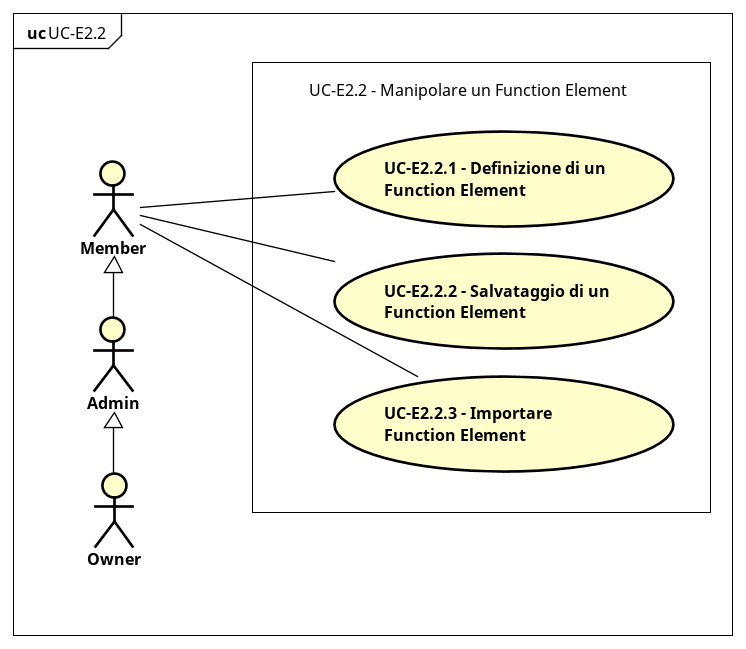
\includegraphics[width=12cm]{res/img/UCEditor/UC-E2.2.png}
      \caption{UC-E2.2 - Manipolare un \glossaryItem{Function Element}}
      \end{center} 
    \end{figure}

    %Tabella 
    \begin{center}
      \bgroup
      \def\arraystretch{1.8}     
      \begin{longtable}{  p{3.5cm} | p{8cm} } 
        
        \hline
        \multicolumn{2}{ | c | }{ \cellcolor[gray]{0.9} \textbf{UC-E2.2 - Manipolare un \glossaryItem{Function Element}}} \\ 
        \hline
        
        \textbf{Attori Primari} &  \glossaryItem{Member}, \glossaryItem{Admin}, \glossaryItem{Owner} \\ 
        \textbf{Scopo e Descrizione} & Viene data la possibilit\`a all'utente di creare, salvare o importare un \glossaryItem{Function Element} collegabile ad un attributo del \glossaryItem{DSL Element}. \\ 
        
        \textbf{Precondizioni}  & L'editor \`e pronto per l'utilizzo. \\ 
        
        \textbf{Postcondizioni} & L'utente ha creato, salvato o importato uno specifico \glossaryItem{Function Element}. \\ 
        \textbf{Scenario principale} & 1. L'utente ha la possibilit\`a di definire un \glossaryItem{Function Element} (UC-E2.2.1)
        
2. L'utente ha la possibilit\`a di salvare \glossaryItem{Function Element}. (UC-E2.2.2)

3. L'utente ha la possibilit\`a di importare \glossaryItem{Function Element}. (UC-E2.2.3)  \\
      \end{longtable}
      \egroup
    \end{center}
\subsubsection{Definizione di un Function Element}

    %Tabella 
    \begin{center}
      \bgroup
      \def\arraystretch{1.8}     
      \begin{longtable}{  p{3.5cm} | p{8cm} } 
        
        \hline
        \multicolumn{2}{ | c | }{ \cellcolor[gray]{0.9} \textbf{UC-E2.2.1 - Definizione di un \glossaryItem{Function Element}}} \\ 
        \hline
        
        \textbf{Attori Primari} &  \glossaryItem{Member}, \glossaryItem{Admin}, \glossaryItem{Owner} \\ 
        \textbf{Scopo e Descrizione} & L'utente ha la possibilit\`a di definire all'interno di un \glossaryItem{Function Element} una funzione nella sintassi del \glossaryItem{DSL}. \\ 
        
        \textbf{Precondizioni}  & L'utente sta visualizzando il form di compilazione di un \glossaryItem{Function Element}. \\ 
        
        \textbf{Postcondizioni} & L'utente ha definito con successo una funzione per il \glossaryItem{Function Element}.\\
        \textbf{Scenario principale} & 1. L'utente definisce all'interno di un \glossaryItem{Function Element} una funzione nella sintassi del \glossaryItem{DSL}. \\ 
      \end{longtable}
      \egroup
    \end{center}

\subsubsection{Salvataggio di un Function Element}

    %Tabella 
    \begin{center}
      \bgroup
      \def\arraystretch{1.8}     
      \begin{longtable}{  p{3.5cm} | p{8cm} } 
        
        \hline
        \multicolumn{2}{ | c | }{ \cellcolor[gray]{0.9} \textbf{UC-E2.2.2 - Salvataggio di un \glossaryItem{Function Element}}} \\ 
        \hline
        
        \textbf{Attori Primari} &  \glossaryItem{Member}, \glossaryItem{Admin}, \glossaryItem{Owner} \\ 
        \textbf{Scopo e Descrizione} & L'utente ha la possibilit\`a di salvare il \glossaryItem{Function Element} creato. \\ 
        
        \textbf{Precondizioni}  & L'utente ha inserito un \glossaryItem{Function Element} valido \\ 
        
        \textbf{Postcondizioni} & Il \glossaryItem{Function Element} \`e stata salvato con successo nel sistema.\\
        \textbf{Scenario principale} & 1. L'utente salva il \glossaryItem{Function Element} creato. \\ 
      \end{longtable}
      \egroup
    \end{center}
    
    
\subsubsection{Importare un Function Element}

    %Tabella 
    \begin{center}
      \bgroup
      \def\arraystretch{1.8}     
      \begin{longtable}{  p{3.5cm} | p{8cm} } 
        
        \hline
        \multicolumn{2}{ | c | }{ \cellcolor[gray]{0.9} \textbf{UC-E2.2.3 - Importare un \glossaryItem{Function Element}}} \\ 
        \hline
        
        \textbf{Attori Primari} &  \glossaryItem{Member}, \glossaryItem{Admin}, \glossaryItem{Owner} \\ 
        \textbf{Scopo e Descrizione} & Il sistema permette di importare un \glossaryItem{Function Element} precedentemente definito.\\ 
        
        \textbf{Precondizioni}  & Il sistema fornisce i \glossaryItem{Function Element} salvati nel sistema. \\ 
        
        \textbf{Postcondizioni} & L'utente ha caricato il \glossaryItem{Function Element} con successo. \\ 
        \textbf{Scenario principale} & 1. L'utente importa un \glossaryItem{Function Element} precedentemente definito.\\
      \end{longtable}
      \egroup
    \end{center}
    
    
\subsubsection{Manipolare un Index Element}
    \begin{figure}[H]
      \begin{center}
        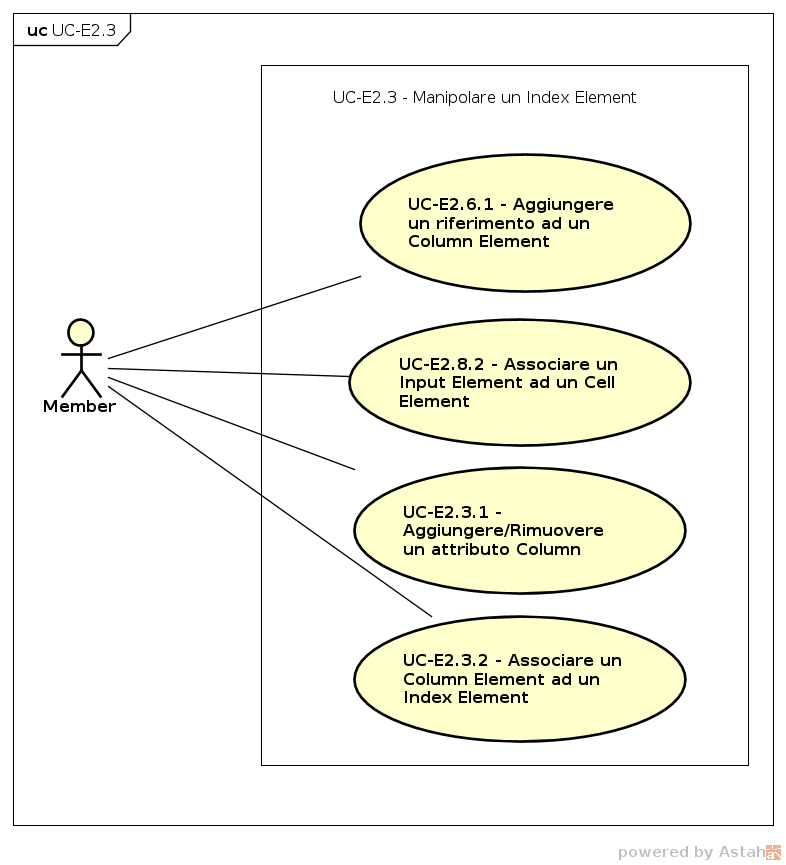
\includegraphics[width=12cm]{res/img/UCEditor/UC-E2.3.png}
      \caption{UC-E2.3 - \glossaryItem{Index Element}}
      \end{center} 
    \end{figure}

    %Tabella 
    \begin{center}
      \bgroup
      \def\arraystretch{1.8}     
      \begin{longtable}{  p{3.5cm} | p{8cm} } 
        
        \hline
        \multicolumn{2}{ | c | }{ \cellcolor[gray]{0.9} \textbf{UC-E2.3 - Manipolare un \glossaryItem{Index Element}}} \\ 
        \hline
        
        \textbf{Attori Primari} &  \glossaryItem{Member}, \glossaryItem{Admin}, \glossaryItem{Owner} \\ 
        \textbf{Scopo e Descrizione} & L'utente ha la possibilit\`a di aggiungere, modificare o eliminare un \glossaryItem{Index Element} \\ 
        
        \textbf{Precondizioni}  & L'utente \`e all'interno dell'editor. \\ 
        
        \textbf{Postcondizioni} & \`E stato manipolato l'\glossaryItem{Index Element} secondo le opzioni indicate dall'utente. \\ 
        \textbf{Scenario Principale} & 1. L'utente pu\`o aggiungere un riferimento ad un \glossaryItem{Column Element}. (UC-E2.6.1)
        
2. L'utente pu\`o associare un \glossaryItem{Input Element}. (UC-E2.8.2)

3. L'utente pu\`o aggiungere/rimuovere un attributo \glossaryItem{Column}. (UC-E2.3.1)

4. L'utente ha la possibilit\'a di associare un \glossaryItem{Column Element}. (UC-E2.3.2)
      \end{longtable}
      \egroup
    \end{center}
\subsubsection{Aggiungere/Rimuovere un attributo Column}

    %Tabella 
    \begin{center}
      \bgroup
      \def\arraystretch{1.8}     
      \begin{longtable}{  p{3.5cm} | p{8cm} } 
        
        \hline
        \multicolumn{2}{ | c | }{ \cellcolor[gray]{0.9} \textbf{UC-E2.3.1 - Aggiungere/Rimuovere un attributo \glossaryItem{Column}}} \\ 
        \hline
        
        \textbf{Attori Primari} &  \glossaryItem{Member}, \glossaryItem{Admin}, \glossaryItem{Owner} \\ 
        \textbf{Scopo e Descrizione} & L'utente ha la possibilit\`a di rimuovere o aggiungere dall'\glossaryItem{Index Element} un attributo \glossaryItem{Column}. \\ 
        
        \textbf{Precondizioni}  &  L'utente \`e all'interno dell'editor e sta visualizzando un \glossaryItem{Index Element} da modificare. \\ 
        
        \textbf{Postcondizioni} & Il sistema aggiunge un attributo \glossaryItem{Column} all'\glossaryItem{Index Element} modificato.\\
        \textbf{Scenario principale} & 1. L'utente rimuove o aggiunge dall'\glossaryItem{Index Element} un attributo \glossaryItem{Column}. \\
      \end{longtable}
      \egroup
    \end{center}
\subsubsection{Associare un Column Element ad un Index Element}

    %Tabella 
    \begin{center}
      \bgroup
      \def\arraystretch{1.8}     
      \begin{longtable}{  p{3.5cm} | p{8cm} } 
        
        \hline
        \multicolumn{2}{ | c | }{ \cellcolor[gray]{0.9} \textbf{UC-E2.3.2 - Associare un \glossaryItem{Column Element} ad un \glossaryItem{Index Element}}} \\ 
        \hline
        
        \textbf{Attori Primari} &  \glossaryItem{Member}, \glossaryItem{Admin}, \glossaryItem{Owner} \\ 
        \textbf{Scopo e Descrizione} & L'utente ha la possibilit\`a di associare un \glossaryItem{Column Element} ad un attributo \glossaryItem{Column} di un \glossaryItem{Index Element}. \\ 
        
        \textbf{Precondizioni}  & L'utente visualizza un \glossaryItem{Index Element} a cui associare il \glossaryItem{Column Element}. \\ 
        
        \textbf{Postcondizioni} & Il sistema associa correttamente il \glossaryItem{Column Element} all' \glossaryItem{Index Element} indicato dall'utente.\\
        \textbf{Scenario principale} & 1. L'utente associa un \glossaryItem{Column Element} ad un attributo \glossaryItem{Column} di un \glossaryItem{Index Element}. \\ 
      \end{longtable}
      \egroup
    \end{center}
    
    
\subsubsection{Manipolazione di un Column Element}

    %Tabella 
    \begin{center}
      \bgroup
      \def\arraystretch{1.8}     
      \begin{longtable}{  p{3.5cm} | p{8cm} } 
        
        \hline
        \multicolumn{2}{ | c | }{ \cellcolor[gray]{0.9} \textbf{UC-E2.4 - Manipolazione di un \glossaryItem{Column Element}}} \\ 
        \hline
        
        \textbf{Attori Primari} &  \glossaryItem{Member}, \glossaryItem{Admin}, \glossaryItem{Owner} \\ 
        \textbf{Scopo e Descrizione} & L'utente ha la possibilit\`a di aggiungere, rimuovere o modificare un \glossaryItem{Column Element} \\ 
        
        \textbf{Precondizioni}  & L'editor \`e visualizzato dall'utente. \\ 
        
        \textbf{Postcondizioni} & Il sistema compie le operazioni sul \glossaryItem{Column Element} indicato dall'utente.\\
        \textbf{Scenario principale} & 1. L'utente aggiunge, rimuove o modifica un \glossaryItem{Column Element} \\ 
      \end{longtable}
      \egroup
    \end{center}
    
\subsubsection{Manipolazione di Row Element}

    %Tabella 
    \begin{center}
      \bgroup
      \def\arraystretch{1.8}     
      \begin{longtable}{  p{3.5cm} | p{8cm} } 
        
        \hline
        \multicolumn{2}{ | c | }{ \cellcolor[gray]{0.9} \textbf{UC-E2.5 - Manipolazione di \glossaryItem{Row Element}}} \\ 
        \hline
        
        \textbf{Attori Primari} &  \glossaryItem{Member}, \glossaryItem{Admin}, \glossaryItem{Owner} \\ 
        \textbf{Scopo e Descrizione} & L'utente ha la possibilit\`a di aggiungere, rimuovere o modificare un \glossaryItem{Row Element}. \\ 
        
        \textbf{Precondizioni}  & L'editor \`e visualizzato dall'utente. \\ 
        
        \textbf{Postcondizioni} & Il sistema compie le operazioni sul \glossaryItem{Row Element} indicato dall'utente.\\
        \textbf{Scenario principale} & 1. L'utente aggiunge, rimuove o modifica un \glossaryItem{Row Element}. \\ 
      \end{longtable}
      \egroup
    \end{center}
\subsubsection{Manipolazione un Document Element}
 

    \begin{figure}[H]
      \begin{center}
        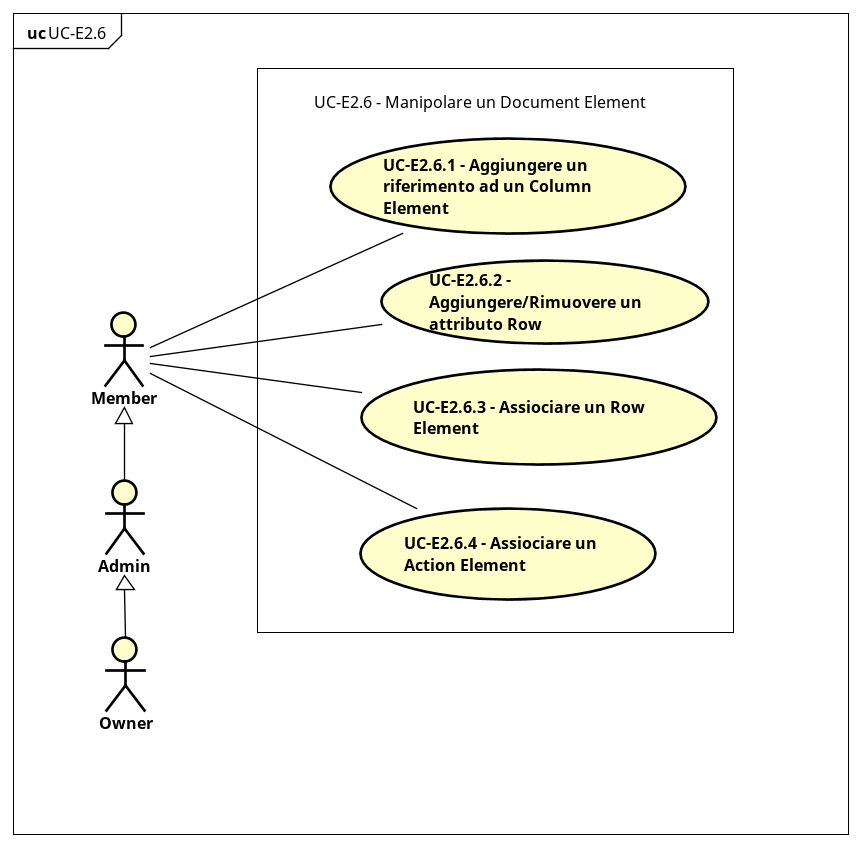
\includegraphics[width=12cm]{res/img/UCEditor/UC-E2.6.png}
      \caption{UC-E2.6 - \glossaryItem{Document Element}}
      \end{center} 
    \end{figure}

    %Tabella 
    \begin{center}
      \bgroup
      \def\arraystretch{1.8}     
      \begin{longtable}{  p{3.5cm} | p{8cm} } 
        
        \hline
        \multicolumn{2}{ | c | }{ \cellcolor[gray]{0.9} \textbf{UC-E2.6 - Manipolazione un \glossaryItem{Document Element}}} \\ 
        \hline
        
        \textbf{Attori Primari} &  \glossaryItem{Member}, \glossaryItem{Admin}, \glossaryItem{Owner} \\ 
        \textbf{Scopo e Descrizione} & L'editor offre la possibilit\`a di manipolare un \glossaryItem{Document Element} agganciandogli altri elementi. \\ 
        
        \textbf{Precondizioni}  & L'utente visualizza l'editor. \\ 
        
        \textbf{Postcondizioni} & Viene generato l'elemento \glossaryItem{Document} nel \glossaryItem{DSL}. \\ 
        \textbf{Scenario Principale} & 1. L'utente ha la possibilit\`a di aggiungere un riferimento ad un \glossaryItem{Column Element}. (UC-E2.6.1)
        
2. L'utente pu\`o aggiungere/rimuovere un attributo \glossaryItem{Row} ad un \glossaryItem{Document Element}. (UC-E2.6.2)

3. L'utente pu\`o associare un \glossaryItem{Row Element} ad un \glossaryItem{Document Element}. (UC-E2.6.3)

4. L'utente pu\`o associare agganciare un \glossaryItem{Action Element} ad un \glossaryItem{Document Element}. (UC-E2.6.4) 
      \end{longtable}
      \egroup
    \end{center}
\subsubsection{Aggiungere un riferimento ad un Column Element}

    %Tabella 
    \begin{center}
      \bgroup
      \def\arraystretch{1.8}     
      \begin{longtable}{  p{3.5cm} | p{8cm} } 
        
        \hline
        \multicolumn{2}{ | c | }{ \cellcolor[gray]{0.9} \textbf{UC-E2.6.1 - Aggiungere un riferimento ad un \glossaryItem{Column Element}}} \\ 
        \hline
        
        \textbf{Attori Primari} &  \glossaryItem{Member}, \glossaryItem{Admin}, \glossaryItem{Owner} \\ 
        \textbf{Scopo e Descrizione} & Si d\`a la possibilit\`a di aggiungere un'associazione per riferimento tra il \glossaryItem{Column Element} e l'attributo \glossaryItem{Populate} del \glossaryItem{Document Element}. \\ 
        
        \textbf{Precondizioni}  & Il \glossaryItem{Document Element} esiste nella sessione corrente dell'editor. \\ 
        
        \textbf{Postcondizioni} & Il sistema aggiunge un riferimento tra il \glossaryItem{Column Element} e il \glossaryItem{Document Element}.\\
        \textbf{Scenario principale} & 1. L'utente aggiunge un'associazione per riferimento tra il \glossaryItem{Column Element} e l'attributo \glossaryItem{Populate} del \glossaryItem{Document Element}. \\ 
      \end{longtable}
      \egroup
    \end{center}
    
    
\subsubsection{Aggiungere/Rimuovere un attributo Row}

    %Tabella 
    \begin{center}
      \bgroup
      \def\arraystretch{1.8}     
      \begin{longtable}{  p{3.5cm} | p{8cm} } 
        
        \hline
        \multicolumn{2}{ | c | }{ \cellcolor[gray]{0.9} \textbf{UC-E2.6.2 - Aggiungere/Rimuovere un attributo \glossaryItem{Row}}} \\ 
        \hline
        
        \textbf{Attori Primari} &  \glossaryItem{Member}, \glossaryItem{Admin}, \glossaryItem{Owner} \\ 
        \textbf{Scopo e Descrizione} & Il sistema dispone la possibilit\`a di aggiungere o rimuovere un attributo \glossaryItem{Row} da un \glossaryItem{Document Element}. \\ 
        
        \textbf{Precondizioni}  & Il \glossaryItem{Document Element} su cui operare l'aggiunta/rimozione di un attributo \glossaryItem{Row} esiste nella sessione corrente dell'editor. \\ 
        
        \textbf{Postcondizioni} & \`E stato manipolato (aggiunto o rimosso) un attributo \glossaryItem{Row} all'interno del \glossaryItem{Document Element}.\\
        \textbf{Scenario principale} & 1. L'utente aggiunge o rimuove un attributo \glossaryItem{Row} da un \glossaryItem{Document Element}. \\
      \end{longtable}
      \egroup
    \end{center}

\subsubsection{Associare un Row Element ad un attributo Row}

    %Tabella 
    \begin{center}
      \bgroup
      \def\arraystretch{1.8}     
      \begin{longtable}{  p{3.5cm} | p{8cm} } 
        
        \hline
        \multicolumn{2}{ | c | }{ \cellcolor[gray]{0.9} \textbf{UC-E2.6.3 - Associare un \glossaryItem{Row Element} ad un attributo \glossaryItem{Row}}} \\ 
        \hline
        
        \textbf{Attori Primari} &  \glossaryItem{Member}, \glossaryItem{Admin}, \glossaryItem{Owner} \\ 
        \textbf{Scopo e Descrizione} & Il sistema dispone la funzionalit\`a per associare un \glossaryItem{Row Element} ad un attributo \glossaryItem{Row} di uno specifico \glossaryItem{Document Element}.  \\ 
        
        \textbf{Precondizioni}  & Il \glossaryItem{Document Element} e il \glossaryItem{Row Element} decisi dall'utente esistono nella sessione corrente dell'editor. \\ 
        
        \textbf{Postcondizioni} & Il sistema ha creato l'associazione tra il \glossaryItem{Row Element} e l'attributo \glossaryItem{Row} del \glossaryItem{Document Element} scelto.\\
        \textbf{Scenario principale} & 1. L'utente associa un \glossaryItem{Row Element} ad un attributo \glossaryItem{Row} di uno specifico \glossaryItem{Document Element}.  \\ 
      \end{longtable}
      \egroup
    \end{center}

\subsubsection{Associare un Action Element a un attributo Row}

    %Tabella 
    \begin{center}
      \bgroup
      \def\arraystretch{1.8}     
      \begin{longtable}{  p{3.5cm} | p{8cm} } 
        
        \hline
        \multicolumn{2}{ | c | }{ \cellcolor[gray]{0.9} \textbf{UC-E2.6.4 - Associare un \glossaryItem{Action Element} a un attributo \glossaryItem{Row}}} \\ 
        \hline
        
        \textbf{Attori Primari} &  \glossaryItem{Member}, \glossaryItem{Admin}, \glossaryItem{Owner} \\ 
        \textbf{Scopo e Descrizione} & Il sistema dispone la funzionalit\`a di associare un \glossaryItem{Action Element} ad un attributo \glossaryItem{Row} di un \glossaryItem{Document Element}. \\ 
        
        \textbf{Precondizioni}  & Il \glossaryItem{Document Element} con il relativo attributo \glossaryItem{Row} esistono nella sessione corrente. \\ 
        
        \textbf{Postcondizioni} & Viene creata un'associazione tra \glossaryItem{Action Element} e l'attributo \glossaryItem{Row} del \glossaryItem{Document Element} indicato dall'utente. \\
        \textbf{Scenario principale} & 1. L'utente associa un \glossaryItem{Action Element} ad un attributo \glossaryItem{Row} di un \glossaryItem{Document Element}. \\ 
      \end{longtable}
      \egroup
    \end{center}
\subsubsection{Manipolazione di un Input Element}
 

    \begin{figure}[H]
      \begin{center}
        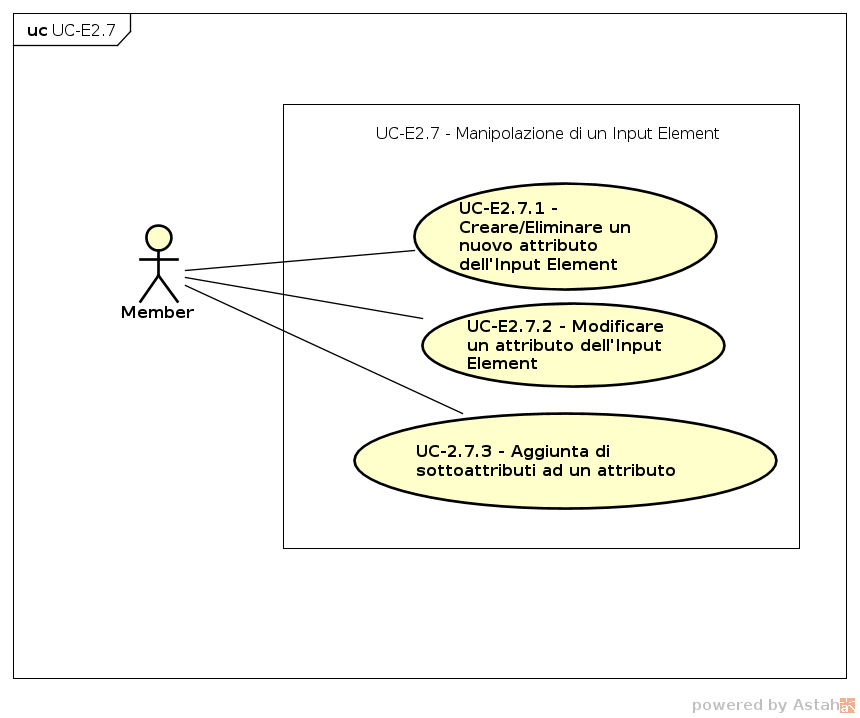
\includegraphics[width=12cm]{res/img/UCEditor/UC-E2.7.png}
      \caption{UC-E2.7 - \glossaryItem{Input Element}}
      \end{center} 
    \end{figure}

    %Tabella 
    \begin{center}
      \bgroup
      \def\arraystretch{1.8}     
      \begin{longtable}{  p{3.5cm} | p{8cm} } 
        
        \hline
        \multicolumn{2}{ | c | }{ \cellcolor[gray]{0.9} \textbf{UC-E2.7 - Manipolazione di un \glossaryItem{Input Element}}} \\ 
        \hline
        
        \textbf{Attori Primari} &  \glossaryItem{Member}, \glossaryItem{Admin}, \glossaryItem{Owner} \\ 
        \textbf{Scopo e Descrizione} & Il sistema da la possibilit\`a all'utente di modificare un \glossaryItem{Input Element} agendo  sui suoi attributi.  \\ 
        
        \textbf{Precondizioni}  & L'utente si trova in una sessione dell'editor valida. \\ 
        
        \textbf{Postcondizioni} & Il sistema ha eseguito le operazioni indicate dall'utente. \\ 
        \textbf{Scenario Principale} & 1. L'utente pu\`o creare/eliminare un nuovo attributo per l'\glossaryItem{Input Element}. (UC-E2.7.1)

2. L'utente pu\`o modificare un attributo dell'\glossaryItem{Input Element}. (UC-E2.7.2)

3. L'utente pu\`o aggiungere ad un attributo dei sottoattributi. (UC-E2.7.3)
      \end{longtable}
      \egroup
    \end{center}
\subsubsection{Creare/Eliminare un nuovo attributo dell'Input Element}

    %Tabella 
    \begin{center}
      \bgroup
      \def\arraystretch{1.8}     
      \begin{longtable}{  p{3.5cm} | p{8cm} } 
        
        \hline
        \multicolumn{2}{ | c | }{ \cellcolor[gray]{0.9} \textbf{UC-E2.7.1 - Creare/Eliminare un nuovo attributo dell'\glossaryItem{Input Element}}} \\ 
        \hline
        
        \textbf{Attori Primari} &  \glossaryItem{Member}, \glossaryItem{Admin}, \glossaryItem{Owner} \\ 
        \textbf{Scopo e Descrizione} & Il sistema fornisce le operazioni di creazione ed eliminazione di un attributo di un \glossaryItem{Input Element} selezionato. \\ 
        
        \textbf{Precondizioni}  & L'utente si è riferito a un \glossaryItem{Input Element} presente nella sessione corrente dell'editor. \\ 
        
        \textbf{Postcondizioni} & Il sistema agisce sull'\glossaryItem{Input Element} aggiungendo o rimuovendo un attributo.\\
        \textbf{Scenario principale} & 1. L'utente crea/elimina un attributo di un \glossaryItem{Input Element} selezionato. \\ 
      \end{longtable}
      \egroup
    \end{center}
\subsubsection{Modificare un attributo dell'Input Element}

    %Tabella 
    \begin{center}
      \bgroup
      \def\arraystretch{1.8}     
      \begin{longtable}{  p{3.5cm} | p{8cm} } 
        
        \hline
        \multicolumn{2}{ | c | }{ \cellcolor[gray]{0.9} \textbf{UC-E2.7.2 - Modificare un attributo dell'\glossaryItem{Input Element}}} \\ 
        \hline
        
        \textbf{Attori Primari} &  \glossaryItem{Member}, \glossaryItem{Admin}, \glossaryItem{Owner} \\ 
        \textbf{Scopo e Descrizione} & L'utente ha la possibilit\`a di modificare la chiave o il valore di un attributo dell'\glossaryItem{Input Element}. \\ 
        
        \textbf{Precondizioni}  & L'\glossaryItem{Input Element} selezionato dall'utente possiede l'attributo da modificare. \\ 
        
        \textbf{Postcondizioni} & Il sistema ha modificato la chiave o il valore dell'attributo selezionato dall'utente.\\
        \textbf{Scenario principale} & 1. L'utente modifica la chiave o il valore di un attributo dell'\glossaryItem{Input Element}. \\ 
      \end{longtable}
      \egroup
    \end{center}
\subsubsection{Aggiunta di sottoattributi ad un attributo}

    %Tabella 
    \begin{center}
      \bgroup
      \def\arraystretch{1.8}     
      \begin{longtable}{  p{3.5cm} | p{8cm} } 
        
        \hline
        \multicolumn{2}{ | c | }{ \cellcolor[gray]{0.9} \textbf{UC-E2.7.3 - Aggiunta di sottoattributi ad un attributo}} \\ 
        \hline
        
        \textbf{Attori Primari} &  \glossaryItem{Member}, \glossaryItem{Admin}, \glossaryItem{Owner} \\ 
        \textbf{Scopo e Descrizione} & L'utente ha la possibilit\`a di poter definire strutture complesse associate ad un attributo. \\ 
        
        \textbf{Precondizioni}  & L'\glossaryItem{Input Element} che possiede l'attributo da espandere esiste nella sessione corrente dell'editor. \\ 
        
        \textbf{Postcondizioni} & Il sistema ha memorizzato la struttura complessa associata all'attributo selezionato dall'utente.\\
        \textbf{Scenario principale} & 1. L'utente definisce strutture complesse associate ad un attributo. \\ 
      \end{longtable}
      \egroup
    \end{center}

\subsubsection{Manipolazione di un Cell Element}
 

    \begin{figure}[H]
      \begin{center}
        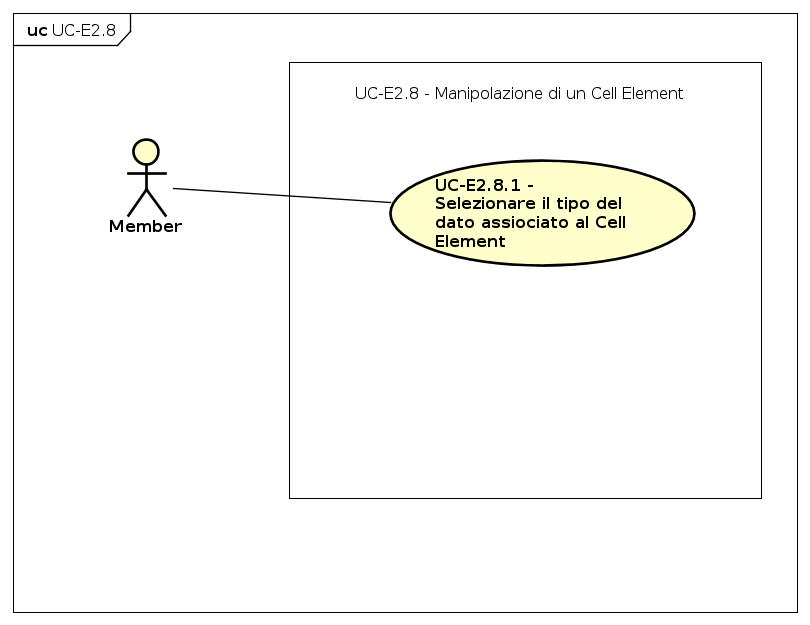
\includegraphics[width=12cm]{res/img/UCEditor/UC-E2.8.png}
      \caption{UC-E2.8 - \glossaryItem{Cell Element}}
      \end{center} 
    \end{figure}

    %Tabella 
    \begin{center}
      \bgroup
      \def\arraystretch{1.8}     
      \begin{longtable}{  p{3.5cm} | p{8cm} } 
        
        \hline
        \multicolumn{2}{ | c | }{ \cellcolor[gray]{0.9} \textbf{UC-E2.8 - Manipolazione di un \glossaryItem{Cell Element}}} \\ 
        \hline
        
        \textbf{Attori Primari} &  \glossaryItem{Member}, \glossaryItem{Admin}, \glossaryItem{Owner} \\ 
        \textbf{Scopo e Descrizione} & L'applicazione fornisce i metodi per definire un \glossaryItem{Cell Element} valido. \\ 
        
        \textbf{Precondizioni}  & L'utente sta visualizzando l'editor. \\ 
        
        \textbf{Postcondizioni} & Il sistema espone il \glossaryItem{Cell Element} valido appena definito. \\ 
        \textbf{Scenario Principale} &  1. Selezionare il tipo del dato associato al \glossaryItem{Cell Element}. (UC-E2.8.1)
      \end{longtable}
      \egroup
    \end{center}
    
    
    
\subsubsection{Selezionare il tipo del dato associato al Cell Element}

    %Tabella 
    \begin{center}
      \bgroup
      \def\arraystretch{1.8}     
      \begin{longtable}{  p{3.5cm} | p{8cm} } 
        
        \hline
        \multicolumn{2}{ | c | }{ \cellcolor[gray]{0.9} \textbf{UC-E2.8.1 - Selezionare il tipo del dato associato al \glossaryItem{Cell Element}}} \\ 
        \hline
        
        \textbf{Attori Primari} &  \glossaryItem{Member}, \glossaryItem{Admin}, \glossaryItem{Owner} \\ 
        \textbf{Scopo e Descrizione} & L'utente pu\`o indicare il tipo di dato da visualizzare tra:
a. string;

b. number;

c. link;

d. image;

e. date. \\ 
        
        \textbf{Precondizioni}  & Il \glossaryItem{Cell Element} su cui si vuole operare esiste nella sessione attiva dell'editor. \\ 
        
        \textbf{Postcondizioni} & Il sistema memorizza il tipo di dato per il \glossaryItem{Cell Element}. \\
        \textbf{Scenario principale} & 1. L'utente seleziona il tipo di dato per \glossaryItem{Cell Element}.  \\
      \end{longtable}
      \egroup
    \end{center}

\subsubsection{Manipolazione di un Dashboard Element}
 

    \begin{figure}[H]
      \begin{center}
        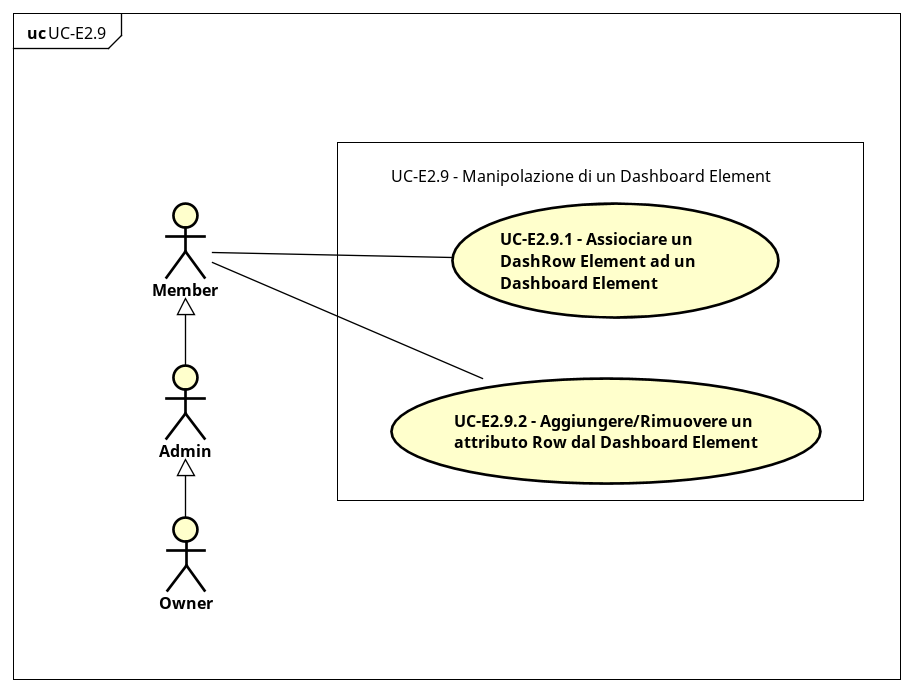
\includegraphics[width=12cm]{res/img/UCEditor/UC-E2.9.png}
      \caption{UC-E2.9 - Manipolazione di un \glossaryItem{Dashboard Element}.}
      \end{center} 
    \end{figure}

    %Tabella 
    \begin{center}
      \bgroup
      \def\arraystretch{1.8}     
      \begin{longtable}{  p{3.5cm} | p{8cm} } 
        
        \hline
        \multicolumn{2}{ | c | }{ \cellcolor[gray]{0.9} \textbf{UC-E2.9 - Manipolazione di un \glossaryItem{Dashboard Element}}} \\ 
        \hline
        
        \textbf{Attori Primari} &  \glossaryItem{Member}, \glossaryItem{Admin}, \glossaryItem{Owner} \\ 
        \textbf{Scopo e Descrizione} & L'utente ha la possibilit\`a di manipolare un \glossaryItem{Dashboard Element}. \\ 
        
        \textbf{Precondizioni}  & L'utente sta visualizzando l'editor. \\ 
        
        \textbf{Postcondizioni} & Il sistema ha memorizzato una definizione valida per il \glossaryItem{Dashboard Element}. \\ 
        \textbf{Scenario Principale} & 1. L'utente pu\`o associare un \glossaryItem{DashRow Element} ad un \glossaryItem{Dashboard Element}. (UC-E2.9.1)
        
2. L'utente pu\`o aggiungere/rimuovere un attributo \glossaryItem{Row} dal \glossaryItem{Dashboard Element}. (UC-E2.9.2)
      \end{longtable}
      \egroup
    \end{center}
    
    
\subsubsection{Associare un DashRow Element ad un Dashboard Element}

    %Tabella 
    \begin{center}
      \bgroup
      \def\arraystretch{1.8}     
      \begin{longtable}{  p{3.5cm} | p{8cm} } 
        
        \hline
        \multicolumn{2}{ | c | }{ \cellcolor[gray]{0.9} \textbf{UC-E2.9.1 - Associare un \glossaryItem{DashRow Element} ad un \glossaryItem{Dashboard Element}}} \\ 
        \hline
        
        \textbf{Attori Primari} &  \glossaryItem{Member}, \glossaryItem{Admin}, \glossaryItem{Owner} \\ 
        \textbf{Scopo e Descrizione} & Permette di definire la struttura di una \glossaryItem{Row} e di legarla a una \glossaryItem{Dashboard}. \\ 
        
        \textbf{Precondizioni}  & Il \glossaryItem{Dashboard Element} e il \glossaryItem{DashRow Element} da collegare esistono nella sessione corrente dell'editor. \\ 
        
        \textbf{Postcondizioni} & Il sistema ha memorizzato il collegamento tra l'attributo \glossaryItem{Row} del \glossaryItem{Dashboard Element} e il \glossaryItem{DashRow Element}.\\
        \textbf{Scenario principale} & 1. L'utente definisce la struttura di una \glossaryItem{Row} e la collega a una \glossaryItem{Dashboard}. \\ 
      \end{longtable}
      \egroup
    \end{center}
\subsubsection{Aggiungere/Rimuovere un attributo Row dal Dashboard Element}

    %Tabella 
    \begin{center}
      \bgroup
      \def\arraystretch{1.8}     
      \begin{longtable}{  p{3.5cm} | p{8cm} } 
        
        \hline
        \multicolumn{2}{ | c | }{ \cellcolor[gray]{0.9} \textbf{UC-E2.9.2 - Aggiungere/Rimuovere un attributo \glossaryItem{Row} dal \glossaryItem{Dashboard Element}}} \\ 
        \hline
        
        \textbf{Attori Primari} &  \glossaryItem{Member}, \glossaryItem{Admin}, \glossaryItem{Owner} \\ 
        \textbf{Scopo e Descrizione} & L'utente pu\`o definire una nuovo attributo \glossaryItem{Row} all'interno della \glossaryItem{Dashboard}. \\ 
        
        \textbf{Precondizioni}  & Il \glossaryItem{Dashboard Element} esiste nella sessione corrente dell'editor. \\ 
        
        \textbf{Postcondizioni} & Il sistema ha aggiunto o rimosso l'attributo \glossaryItem{Row} dalla \glossaryItem{Dashboard Element}.\\
        \textbf{Scenario principale} & 1. L'utente definisce un nuovo attributo \glossaryItem{Row} all'interno della \glossaryItem{Dashboard}. \\
      \end{longtable}
      \egroup
    \end{center}
    
    
\subsubsection{Manipolazione di un DashRow Element}
 

    \begin{figure}[H]
      \begin{center}
        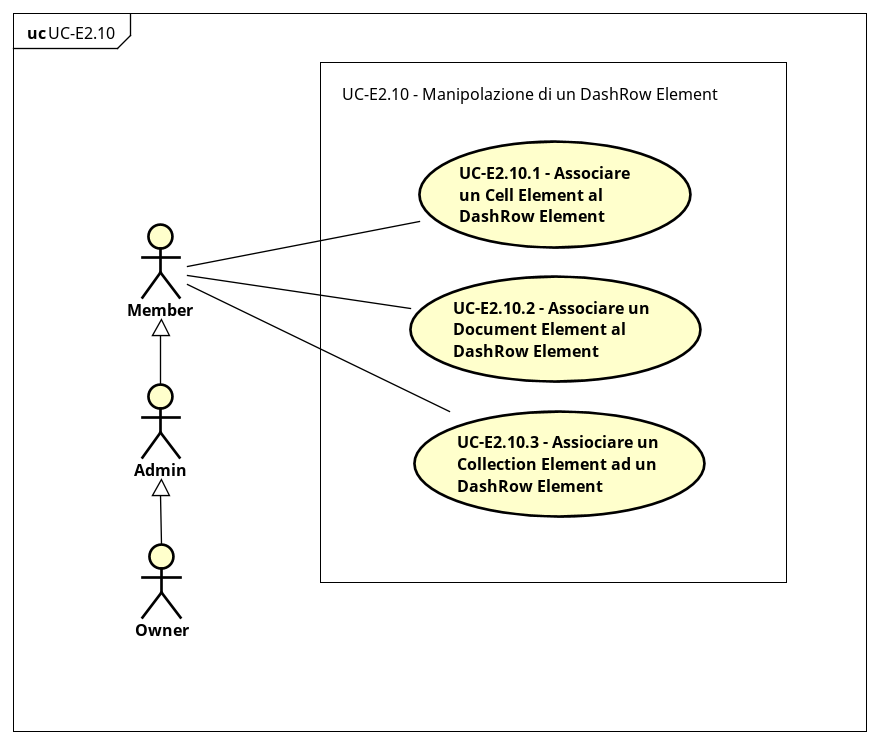
\includegraphics[width=12cm]{res/img/UCEditor/UC-E2.10.png}
      \caption{UC-E2.10 - \glossaryItem{Dash \glossaryItem{Row} Element}}
      \end{center} 
    \end{figure}

    %Tabella 
    \begin{center}
      \bgroup
      \def\arraystretch{1.8}     
      \begin{longtable}{  p{3.5cm} | p{8cm} } 
        
        \hline
        \multicolumn{2}{ | c | }{ \cellcolor[gray]{0.9} \textbf{UC-E2.10 - Manipolazione di un \glossaryItem{DashRow Element}}} \\ 
        \hline
        
        \textbf{Attori Primari} &  \glossaryItem{Member}, \glossaryItem{Admin}, \glossaryItem{Owner} \\ 
        \textbf{Scopo e Descrizione} & Il sistema fornisce i metodi necessari alla manipolazione di un \glossaryItem{DashRow Element}. \\ 
        
        \textbf{Precondizioni}  & Il \glossaryItem{DashRow Element} da manipolare esiste nella sessione corrente dell'editor. \\ 
        
        \textbf{Postcondizioni} & Il sistema ha memorizzato la configurazione del \glossaryItem{DashRow Element}. \\ 
        \textbf{Scenario Principale} & 1. L'utente pu\`o associare un \glossaryItem{Cell Element} al \glossaryItem{DashRow Element}. (UC-E2.10.1)
        
2. L'utente pu\`o associare un \glossaryItem{Document Element} al \glossaryItem{DashRow Element}. (UC-E2.10.2)

3. L'utente pu\`o associare un \glossaryItem{Collection Element} al \glossaryItem{DashRow Element}. (UC-E2.10.3)
      \end{longtable}
      \egroup
    \end{center}
\subsubsection{Associare un Cell Element al DashRow Element}

    %Tabella 
    \begin{center}
      \bgroup
      \def\arraystretch{1.8}     
      \begin{longtable}{  p{3.5cm} | p{8cm} } 
        
        \hline
        \multicolumn{2}{ | c | }{ \cellcolor[gray]{0.9} \textbf{UC-E2.10.1 - Associare un \glossaryItem{Cell Element} al \glossaryItem{DashRow Element}}} \\ 
        \hline
        
        \textbf{Attori Primari} &  \glossaryItem{Member}, \glossaryItem{Admin}, \glossaryItem{Owner} \\ 
        \textbf{Scopo e Descrizione} & Il sistema da la possibilit\`a di associare un \glossaryItem{Cell Element} ad un \glossaryItem{DashRow Element}. \\ 
        
        \textbf{Precondizioni}  & Il \glossaryItem{Cell Element} e il \glossaryItem{DashRow Element} da associare esistono nella sessione corrente dell'editor. \\ 
        
        \textbf{Postcondizioni} & Il sistema ha memorizzato il collegamento tra i due elementi.\\
        \textbf{Scenario principale} & 1. L'utente associa un \glossaryItem{Cell Element} ad un \glossaryItem{DashRow Element}. \\ 
      \end{longtable}
      \egroup
    \end{center}
\subsubsection{Associare un Document Element al DashRow Element}

    %Tabella 
    \begin{center}
      \bgroup
      \def\arraystretch{1.8}     
      \begin{longtable}{  p{3.5cm} | p{8cm} } 
        
        \hline
        \multicolumn{2}{ | c | }{ \cellcolor[gray]{0.9} \textbf{UC-E2.10.2 - Associare un \glossaryItem{Document Element} al \glossaryItem{DashRow Element}}} \\ 
        \hline
        
        \textbf{Attori Primari} &  \glossaryItem{Member}, \glossaryItem{Admin}, \glossaryItem{Owner} \\ 
        \textbf{Scopo e Descrizione} & Il sistema da la possibilit\`a di associare un \glossaryItem{Document Element} ad un \glossaryItem{DashRow Element}. \\ 
        
        \textbf{Precondizioni}  & Il \glossaryItem{Document Element} e il \glossaryItem{DashRow Element} esistono nella sessione corrente dell'editor. \\ 
        
        \textbf{Postcondizioni} & Il sistema ha memorizzato il collegamento tra i due elementi.\\
        \textbf{Scenario principale} & 1. L'utente associa un \glossaryItem{Document Element} ad un \glossaryItem{DashRow Element}. \\ 
      \end{longtable}
      \egroup
    \end{center}
\subsubsection{Associare un Collection Element ad un DashRow Element}

    %Tabella 
    \begin{center}
      \bgroup
      \def\arraystretch{1.8}     
      \begin{longtable}{  p{3.5cm} | p{8cm} } 
        
        \hline
        \multicolumn{2}{ | c | }{ \cellcolor[gray]{0.9} \textbf{UC-E2.10.3 - Associare un \glossaryItem{Collection Element} ad un \glossaryItem{DashRow Element}}} \\ 
        \hline
        
        \textbf{Attori Primari} &  \glossaryItem{Member}, \glossaryItem{Admin}, \glossaryItem{Owner} \\ 
        \textbf{Scopo e Descrizione} & Il sistema da la possibilit\`a di associare un \glossaryItem{Collection Element} ad un \glossaryItem{DashRow Element}. \\ 
        
        \textbf{Precondizioni}  & Il \glossaryItem{Collection Element} e il \glossaryItem{DashRow Element} esistono nella sessione corrente dell'editor. \\ 
        
        \textbf{Postcondizioni} & Il sistema ha memorizzato il collegamento tra i due elementi.\\
        \textbf{Scenario principale} & 1. L'utente associa un \glossaryItem{Collection Element} ad un \glossaryItem{DashRow Element}. \\ 
      \end{longtable}
      \egroup
    \end{center}
\subsubsection{Definire un Action Element}
 

    \begin{figure}[H]
      \begin{center}
        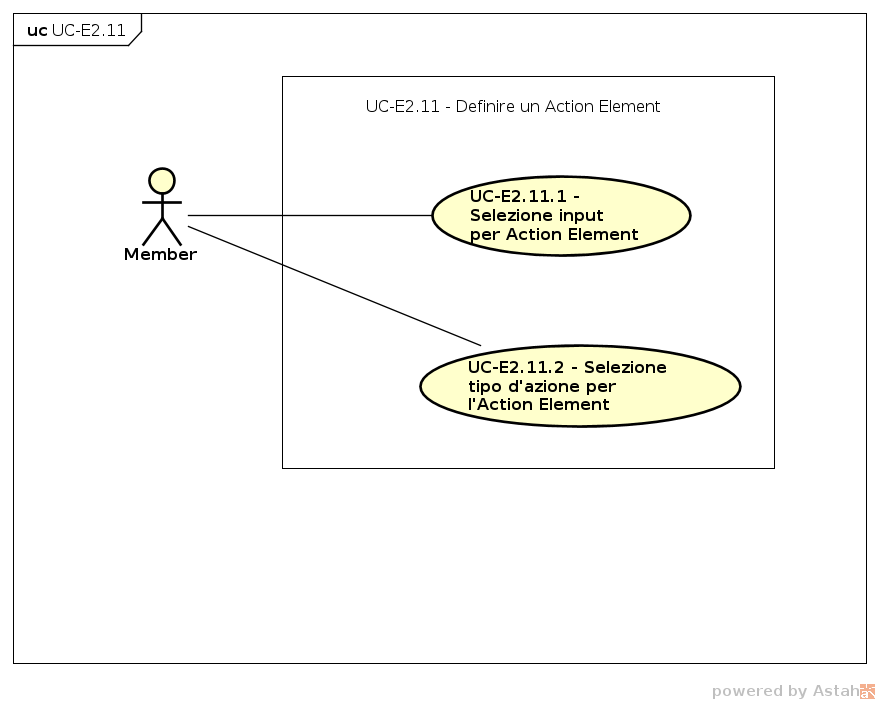
\includegraphics[width=12cm]{res/img/UCEditor/UC-E2.11.png}
      \caption{UC-E2.11 - \glossaryItem{Action Element}}
      \end{center} 
    \end{figure}

    %Tabella 
    \begin{center}
      \bgroup
      \def\arraystretch{1.8}     
      \begin{longtable}{  p{3.5cm} | p{8cm} } 
        
        \hline
        \multicolumn{2}{ | c | }{ \cellcolor[gray]{0.9} \textbf{UC-E2.11 - Definire un \glossaryItem{Action Element}}} \\ 
        \hline
        
        \textbf{Attori Primari} &  \glossaryItem{Member}, \glossaryItem{Admin}, \glossaryItem{Owner} \\ 
        \textbf{Scopo e Descrizione} & Il sistema fornisce le modalit\`a di definizione di un \glossaryItem{Action Element}. \\ 
        
        \textbf{Precondizioni}  & L'utente sta visualizzando l'editor. \\ 
        
        \textbf{Postcondizioni} &  Il sistema ha registrato la definizione dell'\glossaryItem{Action Element}. \\ 
        \textbf{Scenario Principale} & 1. L'utente seleziona un input per l'\glossaryItem{Action Element}. (UC-E2.11.1)
        
2. L'utente seleziona il tipo d'azione per l'\glossaryItem{Action Element}. (UC-E2.11.2) 
      \end{longtable}
      \egroup
    \end{center}
\subsubsection{Selezione input per Action Element}

    %Tabella 
    \begin{center}
      \bgroup
      \def\arraystretch{1.8}     
      \begin{longtable}{  p{3.5cm} | p{8cm} } 
        
        \hline
        \multicolumn{2}{ | c | }{ \cellcolor[gray]{0.9} \textbf{UC-E2.11.1 - Selezione input per \glossaryItem{Action Element}}} \\ 
        \hline
        
        \textbf{Attori Primari} &  \glossaryItem{Member}, \glossaryItem{Admin}, \glossaryItem{Owner} \\ 
        \textbf{Scopo e Descrizione} & L'utente ha la possibilit\`a di selezionare l'input per l'\glossaryItem{Action Element}. \\ 
        
        \textbf{Precondizioni}  & L'\glossaryItem{Action Element} su cui operare esiste nella sessione corrente dell'editor. \\ 
        
        \textbf{Postcondizioni} & Il sistema ha memorizzato l'input da associare all'\glossaryItem{Action Element}.\\
        \textbf{Scenario principale} & 1. L'utente seleziona l'input per l'\glossaryItem{Action Element}. \\ 
      \end{longtable}
      \egroup
    \end{center}
    
    
\subsubsection{Selezione tipo d'azione per l'Action Element}
    %Tabella 
    \begin{center}
      \bgroup
      \def\arraystretch{1.8}     
      \begin{longtable}{  p{3.5cm} | p{8cm} } 
        
        \hline
        \multicolumn{2}{ | c | }{ \cellcolor[gray]{0.9} \textbf{UC-E2.11.2 - Selezione tipo d'azione per l'\glossaryItem{Action Element}}} \\ 
        \hline
        
        \textbf{Attori Primari} &  \glossaryItem{Member}, \glossaryItem{Admin}, \glossaryItem{Owner} \\ 
        \textbf{Scopo e Descrizione} & L'utente pu\`o definire l'azione legata all'\glossaryItem{Action Element}. \\ 
        
        \textbf{Precondizioni}  & L'azione e l'\glossaryItem{Action Element} da collegare sono presenti nella sessione attiva dell'editor. \\ 
        
        \textbf{Postcondizioni} & Il sistema ha associato l'azione all'\glossaryItem{Action Element}.\\
        \textbf{Scenario principale} & 1. L'utente definisce l'azione legata all'\glossaryItem{Action Element}. \\ 
      \end{longtable}
      \egroup
    \end{center}
    
    
    
\subsubsection{Salvataggio specifica DSL}
     %UC-E3: rivedere perché
     % contiene dettagli tecnici, ossia \glossaryItem{casi} d’uso per i quali non è associato alcun
     % \glossaryItem{attore}

    \begin{figure}[H]
      \begin{center}
        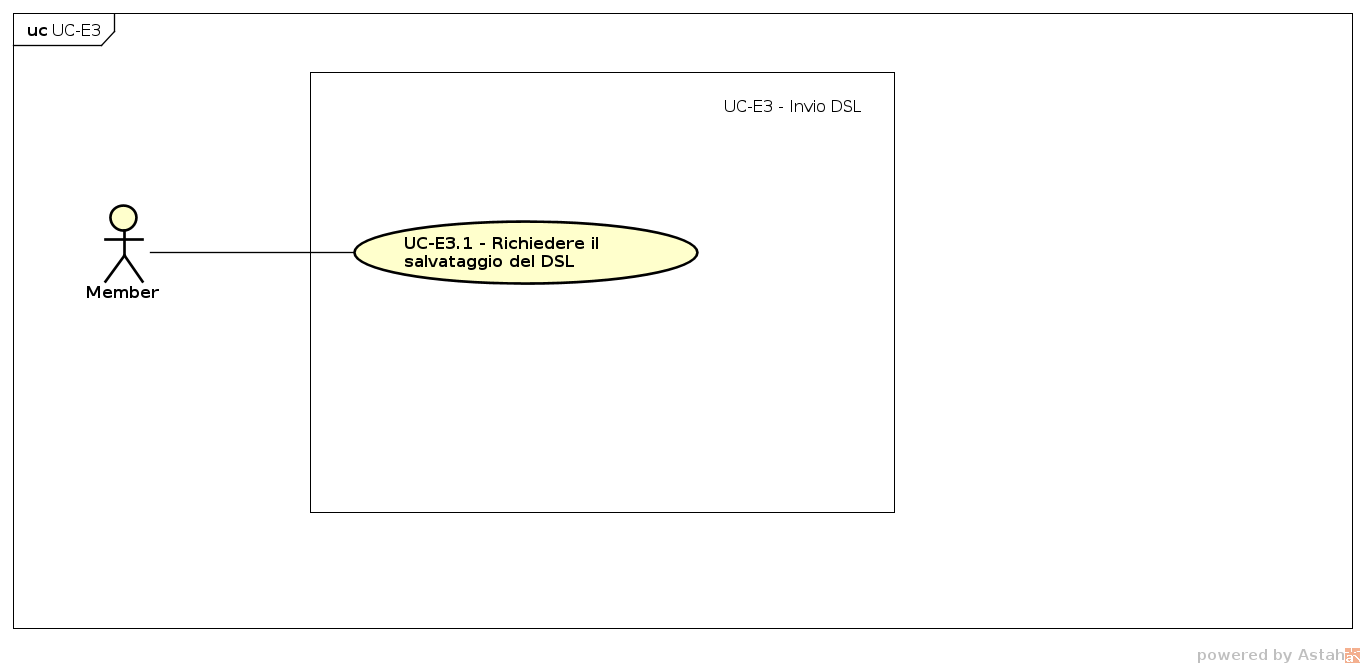
\includegraphics[width=12cm]{res/img/UCEditor/UC-E3.png}
      \caption{UC-E3 - Salvataggio della specifica \glossaryItem{DSL}}
      \end{center} 
    \end{figure}

    %Tabella 
    \begin{center}
      \bgroup
      \def\arraystretch{1.8}     
      \begin{longtable}{  p{3.5cm} | p{8cm} } 
        
        \hline
        \multicolumn{2}{ | c | }{ \cellcolor[gray]{0.9} \textbf{UC-E3 - Salvataggio della specifica \glossaryItem{DSL}}} \\ 
        \hline
        
        \textbf{Attori Primari} &  \glossaryItem{Member}, \glossaryItem{Admin}, \glossaryItem{Owner} \\ 
        \textbf{Scopo e Descrizione} & Il sistema fornisce una modalit\`a di salvataggio per le specifiche \glossaryItem{DSL} definite da un utente. \\ 
        
        \textbf{Precondizioni}  & L'utente visualizza l'editor e ha creato una specifica \glossaryItem{DSL} valida da salvare. \\ 
        
        \textbf{Postcondizioni} & La specifica \glossaryItem{DSL} \`e stata memorizzata con successo nel sistema. \\ 
        \textbf{Scenario Principale} & 1. L'utente richiede il salvataggio del \glossaryItem{DSL}. (UC-E3.1) 
      \end{longtable}
      \egroup
    \end{center}
\subsubsection{Richiedere il salvataggio della specifica DSL}

    %Tabella 
    \begin{center}
      \bgroup
      \def\arraystretch{1.8}     
      \begin{longtable}{  p{3.5cm} | p{8cm} } 
        
        \hline
        \multicolumn{2}{ | c | }{ \cellcolor[gray]{0.9} \textbf{UC-E3.1 - Richiedere il salvataggio della specifica \glossaryItem{DSL}}} \\ 
        \hline
        
        \textbf{Attori Primari} &  \glossaryItem{Member}, \glossaryItem{Admin}, \glossaryItem{Owner} \\ 
        \textbf{Scopo e Descrizione} & L'utente chiede all'applicazione di eseguire le operazioni necessarie affinché la specifica \glossaryItem{DSL} venga salvata ed eseguita con successo. \\ 
        
        \textbf{Precondizioni}  & L'utente visualizza l'editor e ha definito una specifica \glossaryItem{DSL}\\ 
        
        \textbf{Postcondizioni} & Il sistema ha preso in carico la richiesta di salvataggio della specifica \glossaryItem{DSL}.\\
        \textbf{Scenario principale} & 1. L'utente chiede all'applicazione di eseguire le operazioni necessarie affinché la specifica \glossaryItem{DSL} venga salvata ed eseguita con successo. \\ 
      \end{longtable}
      \egroup
    \end{center}
\subsubsection{Validazione del DSL}

    %Tabella 
    \begin{center}
      \bgroup
      \def\arraystretch{1.8}     
      \begin{longtable}{  p{3.5cm} | p{8cm} } 
        
        \hline
        \multicolumn{2}{ | c | }{ \cellcolor[gray]{0.9} \textbf{UC-E3.2 - \glossaryItem{Validazione} del \glossaryItem{DSL}}} \\ 
        \hline
        \textbf{Attori Primari} &  \glossaryItem{Member}, \glossaryItem{Admin}, \glossaryItem{Owner} \\ 
        \textbf{Scopo e Descrizione} & Il sistema esegue i controlli di \glossaryItem{validazione} per il \glossaryItem{DSL} creato. \\ 
        
        \textbf{Precondizioni}  & L'utente ha fatto richiesta di salvataggio del \glossaryItem{DSL} \\ 
        
        \textbf{Postcondizioni} & Il \glossaryItem{DSL} \`e stato correttamente validato. \\ 
        \textbf{Scenario principale} & 1. Il sistema esegue i controlli di \glossaryItem{validazione} per il \glossaryItem{DSL} creato. \\
        \textbf{Estensioni} & 1. Il \glossaryItem{DSL} non \`e valido. (UC-E3.4) \\
      \end{longtable}
      \egroup
    \end{center}
    
    
\subsubsection{Memorizzazione della specifica DSL}

    %Tabella 
    \begin{center}
      \bgroup
      \def\arraystretch{1.8}     
      \begin{longtable}{  p{3.5cm} | p{8cm} } 
        
        \hline
        \multicolumn{2}{ | c | }{ \cellcolor[gray]{0.9} \textbf{UC-E3.3 - Memorizzazione della specifica \glossaryItem{DSL}}} \\ 
        \hline
        \textbf{Attori Primari} &  \glossaryItem{Member}, \glossaryItem{Admin}, \glossaryItem{Owner} \\ 
         \textbf{Scopo e Descrizione} &  Il sistema esegue la \glossaryItem{procedura} di memorizzazione della specifica \glossaryItem{DSL}. \\ 
        
        \textbf{Precondizioni}  & La specifica \glossaryItem{DSL} in input deve essere valida. \\ 
        
        \textbf{Postcondizioni} & La specifica \glossaryItem{DSL} \`e stato correttamente memorizzata nel sistema. \\ 
        \textbf{Scenario principale} & 1. Il sistema esegue la \glossaryItem{procedura} di memorizzazione della specifica \glossaryItem{DSL}. \\
      \end{longtable}
      \egroup
    \end{center}
\subsubsection{La specifica DSL non \`e valida}

    %Tabella 
    \begin{center}
      \bgroup
      \def\arraystretch{1.8}     
      \begin{longtable}{  p{3.5cm} | p{8cm} } 
        
        \hline
        \multicolumn{2}{ | c | }{ \cellcolor[gray]{0.9} \textbf{UC-E3.4 - La specifica \glossaryItem{DSL} non \`e valida}} \\ 
        \hline
        \textbf{Attori Primari} &  \glossaryItem{Member}, \glossaryItem{Admin}, \glossaryItem{Owner} \\ 
        \textbf{Scopo e Descrizione} & Il sistema fornisce un messaggio di errore che evidenzia i punti della specifica \glossaryItem{DSL} non validi. \\ 
        
        \textbf{Precondizioni}  & La specifica \glossaryItem{DSL} non \`e corretto. \\ 
        
        \textbf{Postcondizioni} & L'utente \`e stato avvisato tramite un messaggio della presenza di errori nella specifica \glossaryItem{DSL}.\\
        \textbf{Scenario principale} & 1. L'utente visualizza un messaggio di errore che evidenzia i punti della specifica \glossaryItem{DSL} non validi. \\ 
      \end{longtable}
      \egroup
    \end{center}


    \newpage
